\documentclass[12pt]{article}
% Esenciales:
\usepackage[a4paper, margin=2.5cm]{geometry} % Hoja A4 con margen de 2.5cm
\usepackage{tikz,pgfplots}
\usepackage{graphicx}
\usepackage{float}

% Tipo de letra
% Arial:
\renewcommand{\familydefault}{\sfdefault}
% Comentar Arial y descomentar las siguientes para Helvetica:
% \usepackage{helvet}
% \renewcommand{\familydefault}{\sfdefault}

% Para citas bibliograficas:
\usepackage[backend=bibtex, style=numeric]{biblatex}
\addbibresource{bib/referencias.bib}

% Índice clickeable
% \usepackage[colorlinks=true, linkcolor=black]{hyperref}
\usepackage[
  colorlinks=true,
  linkcolor=black,      % Títulos, referencias internas, índice
  citecolor=black,      % Citas [1], [2], etc.
  urlcolor=blue         % Enlaces web
]{hyperref}

\usepackage[utf8]{inputenc}
\usepackage[T1]{fontenc}
\usepackage{listings}          % Para código
\usepackage{xcolor}            % Para colores


\usepackage{titlesec}   % Para modificar títulos
\usepackage{tocloft}    % Para personalizar el índice
% --- Ocultar números en títulos (pero mantener en índice) ---
\titleformat{\section}
  {\color{cyan!45!black}\normalfont\Large\bfseries}{}{0em}{}

\titleformat{\subsection}
{\color{black}\normalfont\large\bfseries}{}{0em}{}  % Sin número visible y con color
  

% --- Asegurar que el índice muestre los números ---
\renewcommand{\cftsecaftersnum}{.}       % Punto después del número (opcional)
\renewcommand{\cftsubsecaftersnum}{.}    % Ej: "1.2." en el índice       % Carga paquetes
% --- Carga colores si no están en paquetes.tex ---
% --- Paleta VSCode White/Dark ---
% Para el fondo en códigos (255 -> blanco, 0 -> negro):
\definecolor{vsBackground}{RGB}{255, 255, 255}
\definecolor{vsText}{RGB}{0, 0, 0}
\definecolor{vsKeyword}{RGB}{86, 156, 214}
\definecolor{vsComment}{RGB}{80, 153, 85}
\definecolor{vsString}{RGB}{206, 145, 120}
\definecolor{vsLineNumbers}{RGB}{100, 100, 100}

% --- Estilo común (basado en VSCode Dark) ---
\lstdefinestyle{vsDarkStyle}{
    backgroundcolor=\color{vsBackground},
    basicstyle=\ttfamily\color{vsText}\small,
    keywordstyle=\color{vsKeyword},
    commentstyle=\color{vsComment},
    stringstyle=\color{vsString},
    numberstyle=\color{vsLineNumbers},
    showstringspaces=false,
    numbers=left,
    frame=none,
    breaklines=true,
    tabsize=4,
    xleftmargin=15pt,
    escapeinside={(*@}{@*)},
    literate= % Caracteres especiales (¡, ñ, etc.)
      {á}{{\'a}}1 {é}{{\'e}}1 {í}{{\'i}}1 {ó}{{\'o}}1 {ú}{{\'u}}1
      {Á}{{\'A}}1 {É}{{\'E}}1 {Í}{{\'I}}1 {Ó}{{\'O}}1 {Ú}{{\'U}}1
      {ñ}{{\~n}}1 {Ñ}{{\~N}}1
      {¡}{{!`}}1  {¿}{{?`}}1
      {"}{{\textquotedbl}}1
      {°}{{\textdegree}}1
      {|}{{\textbar}}1
      {~}{{\textasciitilde}}1,
}


% --- Lenguajes ---

\lstdefinelanguage{C}{
    style=vsDarkStyle,
    morekeywords={int, float, double, char, bool, true, false, NULL, sizeof, const, struct, typedef},
    morecomment=[l]{//},       % Comentarios de una línea
    morecomment=[s]{/*}{*/},   % Comentarios multilínea
    morestring=[b]{"},         % Strings entre comillas
    sensitive=true,            % Distingue mayúsculas/minúsculas
}

\lstdefinelanguage{JavaScript}{
    style=vsDarkStyle,
    morekeywords={let, const, var, function, if, else, for, while, return, class, import, export, console, async, await},
    morecomment=[l]{//},
    morecomment=[s]{/*}{*/},
    morestring=[b]{"},         % Strings con "
    morestring=[b]{'},         % Strings con '
    sensitive=true,
}

\lstdefinelanguage{Python}{
    style=vsDarkStyle,
    morekeywords={def, class, lambda, with, yield, try, except, import, from, as, self, None, True, False},
    morecomment=[l]{\#},       % Comentarios con #
    morestring=[b]{"},         % Strings con "
    morestring=[b]{'},         % Strings con '
    morestring=[s]{"""}{"""},  % Docstrings
    sensitive=true,
}

\lstdefinelanguage{MATLAB}{
    style=vsDarkStyle,
    morekeywords={function, end, if, else, elseif, for, while, switch, case, otherwise, try, catch, classdef, properties, methods},
    morecomment=[l]{\%},       % Comentarios con %
    morestring=[b]{'},         % Strings con '
    sensitive=false,           % MATLAB no distingue mayúsculas/minúsculas en keywords
} % Carga configs de código
\pgfplotsset{compat=1.18} % Set pgfplots compatibility mode

% ===== Variables editables =====
\newcommand{\materia}{Nombre de la materia}       % Nombre de la materia
\newcommand{\titulo}{PRÁCTICA 2: MODELOS DE PROPAGACIÓN } % Título del trabajo
\newcommand{\profesor}{Noé Torres Cruz}            % Nombre del profesor
\newcommand{\alumno}{\\ Guillén González Carlos Jael}             % Nombre del alumno
\newcommand{\alumnodos}{Rodriguez Gallegos Sara}             % Nombre del alumno
\newcommand{\grupo}{2TM6}
\newcommand{\fecha}{23-06-25}                  % Fecha (puede ser manual: "1 de mayo de 2024")


\begin{document}
% portada_informe.tex
\begin{titlepage}
    % --- Logos en tabla ---
    \noindent
    \begin{tabular}{@{} p{0.5\textwidth} p{0.5\textwidth} @{}}
        
\includegraphics[width=0.8\linewidth]{./img/logo-ipn.png} &
        \hfill 
\includegraphics[width=0.6\linewidth]{./img/logo-upiita.png} \\
    \end{tabular}


    \centering
    \vspace*{1cm}
    {\huge \textbf{Instituto Politécnico Nacional} \par}
    {\LARGE \textbf{Unidad Profesional Interdisciplinaria de Ingeniería y Tecnologías Avanzadas} \par}
    \vspace{1.5cm}
    {\LARGE \textbf{\materia} \par} % Variable: materia
    \vspace{1cm}
    {\Huge \titulo \par}            % Variable: título
    \vspace{2cm}
    {\large \textbf{Profesor:} \profesor \par} % Variable: profesor
    {\large \textbf{Alumnos:} \alumno \par}     % Variable: alumno
    {\large \alumnodos}
    \vfill
    {\large \textbf{\grupo} \par}       % Variable: grupo
    
    {\large \fecha \par}            % Variable: fecha
\end{titlepage}

\tableofcontents
\clearpage
\section{Objetivo}

Analizar y comparar distintos modelos de propagación de señal en sistemas celulares (como el modelo de espacio libre, superficie reflejante, COST231 y lognormal) mediante la implementación de simulaciones y el análisis de datos obtenidos a partir de mediciones reales, con el fin de comprender el comportamiento de la potencia recibida en función de la distancia y las condiciones del entorno, tanto con línea de vista (LoS) como sin línea de vista (NLoS).

\section{\Large Introducción}

La propagación de ondas electromagnéticas es un aspecto fundamental en el dise\~no de redes de comunicación inalámbrica, especialmente en sistemas celulares. Los modelos de propagación permiten predecir cómo se comporta la se\~nal en diferentes condiciones ambientales, topográficas y estructurales. En esta práctica se exploran cuatro modelos fundamentales: Modelo de Espacio Libre, Superficie Reflejante, COST231-Walfish-Ikegami y Lognormal con Ensombrecimiento. Además, se aborda la detección de línea de vista (LoS), un criterio clave en la selección del modelo adecuado.

\subsection{Modelo de Espacio Libre}
Este modelo representa una condición ideal en la que no existen obstrucciones entre el transmisor y el receptor. Se basa en la ley del inverso del cuadrado y describe cómo la potencia disminuye con el cuadrado de la distancia:

\begin{equation}
L\_{fs} = 32.44 + 20\log\_{10}(d\_{km}) + 20\log\_{10}(f\_{MHz})
\end{equation}

\noindent Donde:
\begin{itemize}
\item $L\_{fs}$: Pérdida de trayectoria (dB),
\item $d\_{km}$: Distancia en kilómetros,
\item $f\_{MHz}$: Frecuencia en megahercios.
\end{itemize}

\begin{figure}[H]
\centering
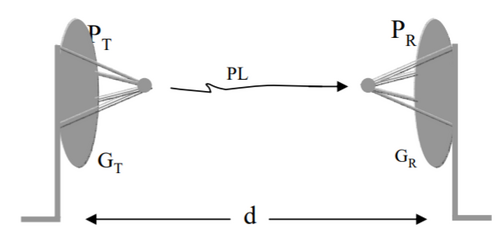
\includegraphics[width=0.5\textwidth]{./img/espaciolibre.png}
\caption{Modelo de espacio libre. La se\~nal viaja sin obstrucciones.}
\end{figure}

\subsection{Modelo de Superficie Reflejante}
Este modelo considera que la se\~nal se refleja en el suelo antes de alcanzar el receptor, generando interferencia constructiva o destructiva:

\begin{equation}
L\_{sr} = 40\log\_{10}(d\ [m]) - 20\log\_{10}(ht)(hr)
\end{equation}

\noindent Donde:
\begin{itemize}
\item $d$: Distancia en metros,
\item $ht$: Altura del transmisor,
\item $hr$: Altura del receptor.
\end{itemize}

\begin{figure}[H]
\centering
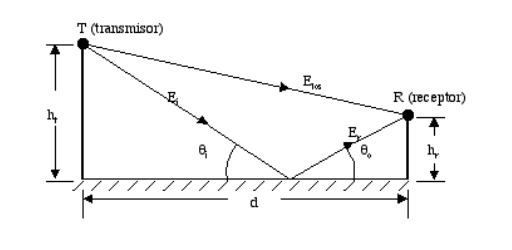
\includegraphics[width=0.5\textwidth]{./img/reflejante.png}
\caption{Modelo con reflexión en superficie terrestre.}
\end{figure}

\subsection{Modelo COST231-Walfish-Ikegami}
Este modelo se usa en entornos urbanos. Considera la influencia de edificios, calles y la geometría urbana. Se divide en pérdidas de trayectoria básica, de techo a calle y por difracción:

\begin{align}
L &= L_0 + L_{rts} + L_{msd} \\
L_0 &= 32.4 + 20\log_{10}(d_{km}) + 20\log_{10}(f_{MHz}) \\
L_{rts} &= -16.9 - 10\log_{10}(w) + 10\log_{10}(f) + 20\log_{10}(h_t - h_r) + L_{ori} \\
L_{msd} &= L_{bsh} + k_a + k_d \log_{10}(d) + k_f \log_{10}(f) - 9 \log_{10}(b)
\end{align}

\noindent Parámetros:
\begin{itemize}
\item $w$: Ancho de calle, $b$: Separación entre edificios,
\item $L_{ori}$: Pérdida por orientación, $L_{bsh}$: Pérdida techo a calle,
\item $k_a = 54$, $k_d = 18$, $k_f$: Factor de frecuencia.
\end{itemize}

\begin{figure}[H]
\centering
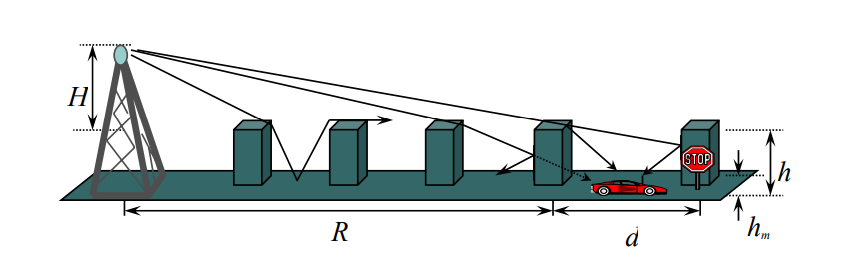
\includegraphics[width=0.5\textwidth]{./img/walfish.png}
\caption{Modelo COST231 considerando estructura urbana.}
\end{figure}

\subsection{Modelo Lognormal con ensombrecimiento}
Este modelo incorpora la variabilidad aleatoria debida a obstrucciones como edificios o árboles. La pérdida total incluye una componente aleatoria:

\begin{equation}
L\_{\log} = 10 \alpha \log\_{10}(d\_{km}) + X\_\sigma
\end{equation}

\noindent Donde:
\begin{itemize}
\item $alpha$: Exponente de pérdida,
\item $X_sigma$: Variable aleatoria normal con desviación $sigma$ (dB).
\end{itemize}

\begin{equation}
P\_{rx} = P\_{tx} + G\_{tx} + G\_{rx} - L\_{\log}
\end{equation}

\subsection{Análisis de Línea de Vista (LoS)}
La detección de LoS se basa en una evaluación geométrica entre la estación base y el receptor. Si un obstáculo (ej. edificio) intersecta la línea entre ambos puntos, se considera NLoS (Non-Line-of-Sight), lo cual modifica el modelo de propagación.

La correcta identificación de la condición LoS permite seleccionar el modelo más adecuado y obtener predicciones más precisas sobre la potencia de la se\~nal recibida.

\clearpage

\section{\Large Desarrollo}

\begin{enumerate}
	\subsection{Obteniendo los datos.}
	\item Ubicar la Estación Base (Base Station - BS), cuya ubicación es 19.503668573568277, -99.1279845883227. Usando Google Maps o por inspección directa estimar la altura a la que se encuentran colocadas las antenas.
	      \begin{figure}[H]
		      \centering
		      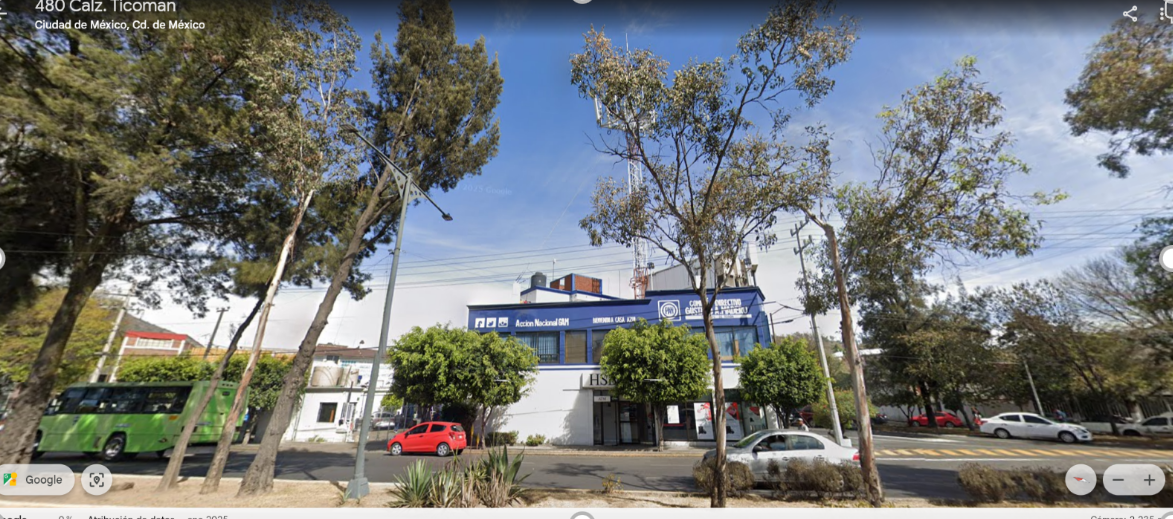
\includegraphics[width=0.9\textwidth]{./img/bs.png}
		      \caption{Imagen de la estación base en las coordenadas dadas.}
		      \label{fig:bs}
	      \end{figure}
	\item Trazar una línea recta entre la BS y la coordenada asignada y calcular la potencia recibida por cada intersección entre una calle y la línea trazada considerando los modelos espacio libre, superficie reflejante, COST231 Walfish-Ikegami y lognormal.
	      \textbf{Coordenadas: 19.508953097456004, -99.12414451054960}
	      \begin{figure}[H]
		      \centering
		      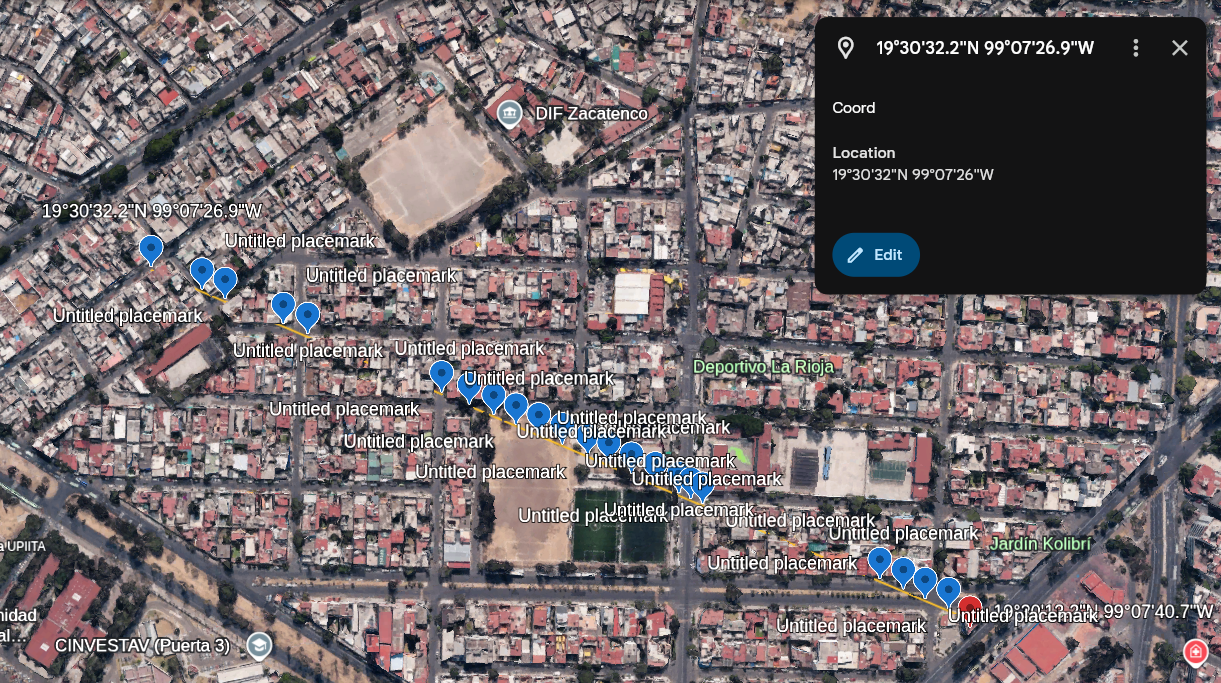
\includegraphics[width=0.9\textwidth]{./img/coordenada-dada.png} % Ajusta el ancho
		      \caption{Línea recta desde la BS hasta la coordenada asignada.}
		      \label{fig:coordenada-dada}
	      \end{figure}

	      \begin{figure}[H]
		      \centering
		      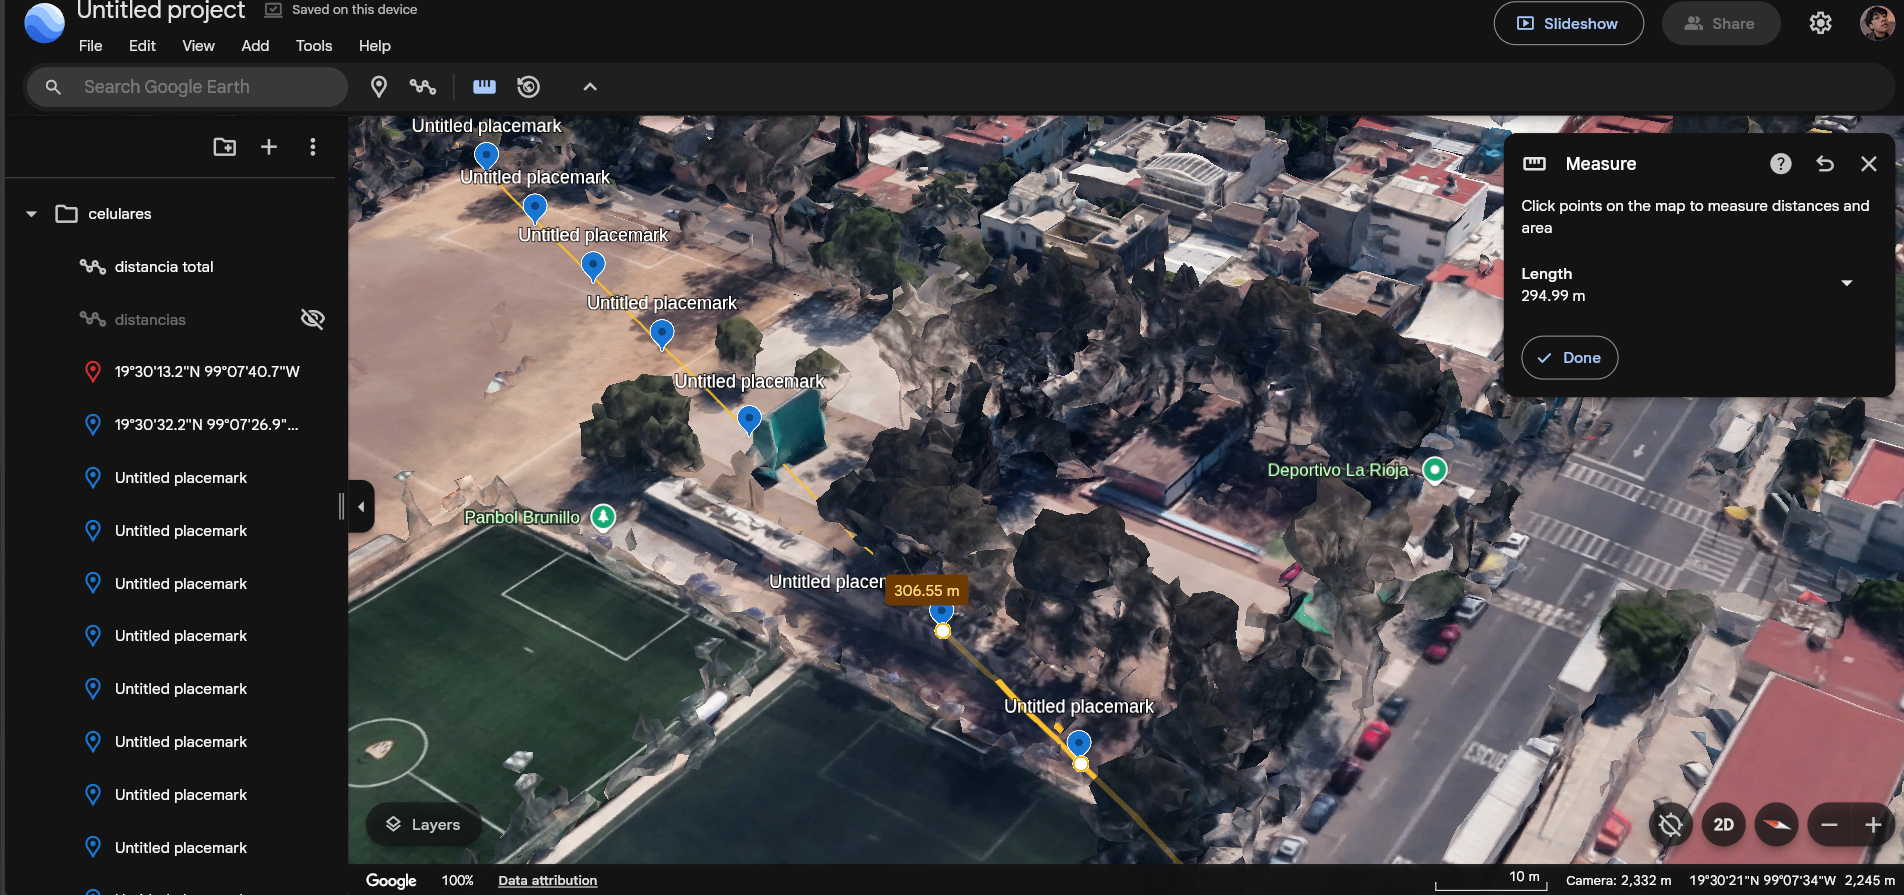
\includegraphics[width=0.9\textwidth]{./img/distancias-puntos.png} % Ajusta el ancho
		      \caption{Sacando las distancias de la BS a cada punto (aprox cada 20m en exteriores).}
		      \label{fig:distancias-puntos}
	      \end{figure}
	      \begin{figure}[H]
		      \centering
		      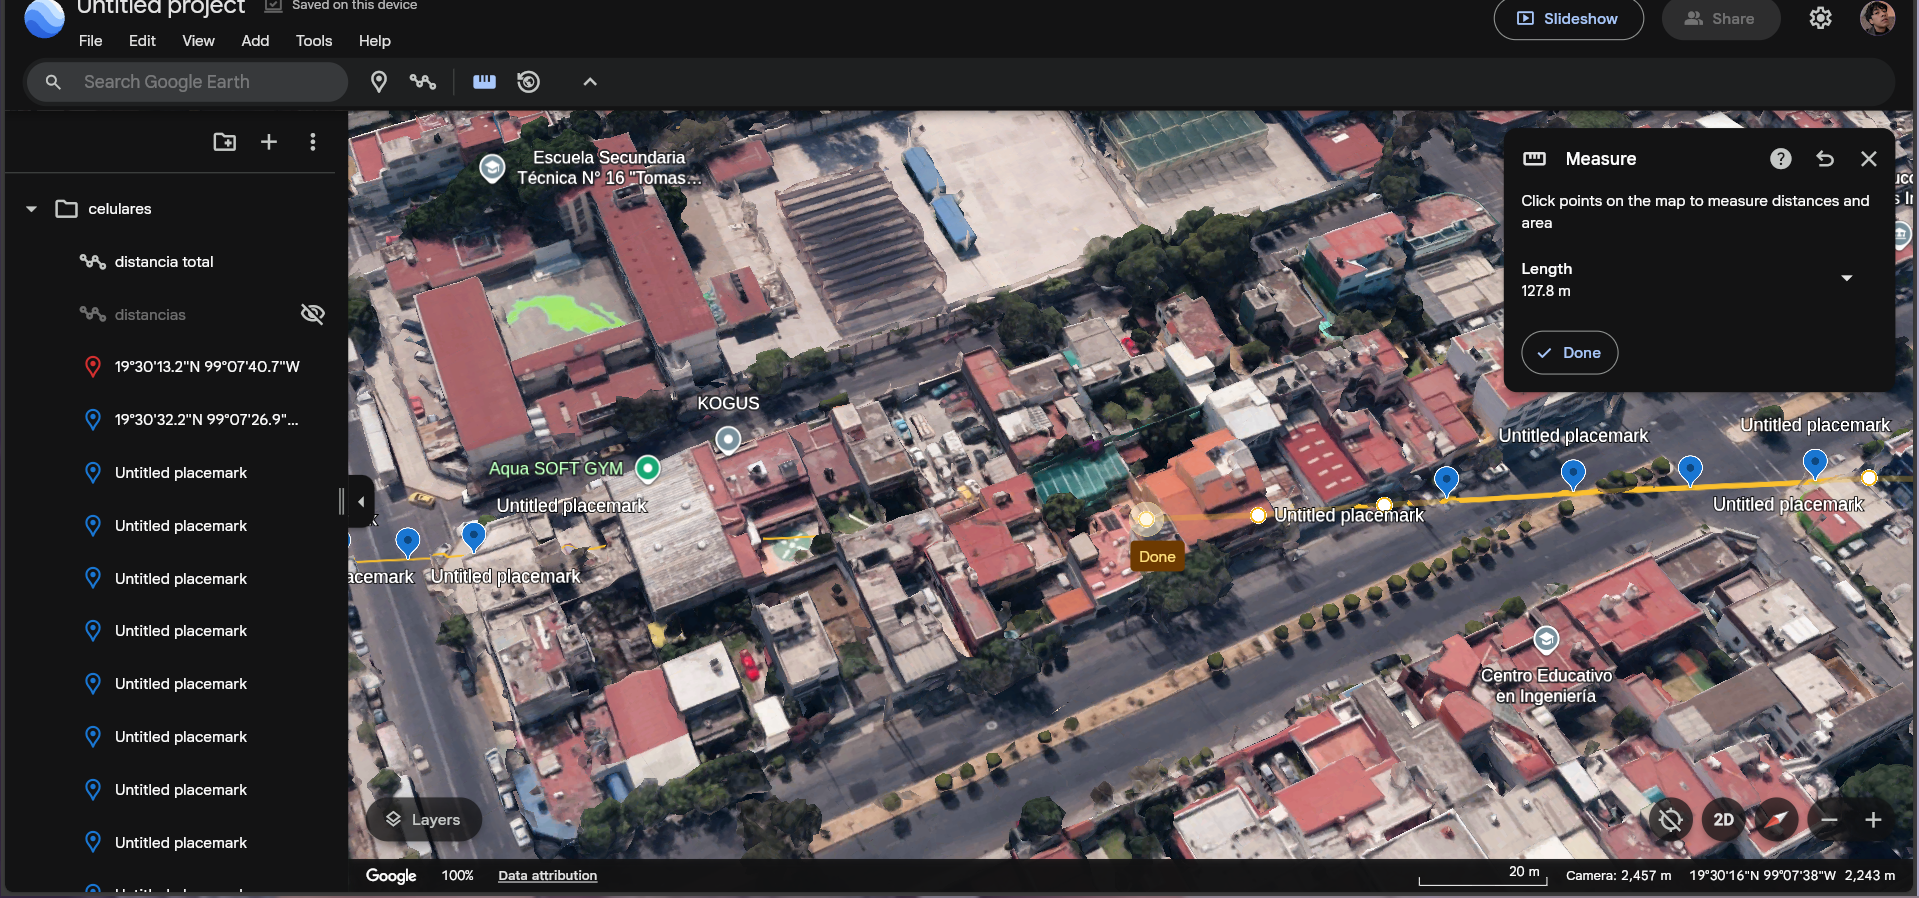
\includegraphics[width=0.9\textwidth]{./img/distancias-edificios.png} % Ajusta el ancho
		      \caption{Sacando las distancias de los edificios.}
		      \label{fig:distancias-edificios}
	      \end{figure}
	\item Considerar una frecuencia de operación de 1,935 MHz para los modelos que lo requieran. Además, considerar que la potencia de transmisión es de 10W y que las ganancias de las antenas transmisora y receptora son 9 y 3 dB, respectivamente.  
	\item Para el modelo COST231 Walfish-Ikegami realizar una tabla con los siguientes datos por cada punto analizado:  
          \begin{enumerate}
            \item Coordenadas 
            \item Distancia a la EB
            \item Si existe LOS o no 
            \item Separación promedio entre edificios, b (si aplica). 
            \item Ancho de la “calle” en la que se encuentra el móvil, w (si aplica). 
            \item Altura promedio de edificios, h (si aplica) 
            \item Ángulo de orientación, $\phi$ (si aplica).
            \item $L_0.$
            \item $L_{rts}$. (Si aplica).
            \item \item $L_{msd}$. (Si aplica).
            \item Potencia recibida (en dBm) 
          \end{enumerate}
                \begin{table}[H]
                \centering
                \begin{tabular}{|c|c|c|c|}
                    \hline
                    Coordenadas & Distancia a la EB & LOS & Potencia recibida (dBm) \\
                    \hline
                    19.50, -99.12 & 100 m & Sí & -80 \\
                    19.51, -99.13 & 120 m & No & -85 \\
                    \hline
                \end{tabular}
                \caption{Ejemplo de tabla para los puntos analizados.}
                \label{tab:ejemplo}
            \end{table}          


\end{enumerate}

\clearpage


\end{document}